\section{Refinement via Maximum Curvature Ratio/Deviation}
One could, for instance, find the maximum value for curvature ratio on the segment to determine whether or not to further subdivide the segment.  This is an example of “deviation-based” refinement.  For a given segment, the maximum curvature ratio is found where the perpendicular distance between the segment and the curve is maximum.  This might not correspond to the point where the combined arc-length of the two new segments is maximally different from the current configuration.  For instance consider the triangle, (\textit{A}, \textit{B}, \textit{C}) with sides of length following the Pythagorean triple (5,12,13) and therefore perimeter of 30.

\begin{figure}[h!]
  \center{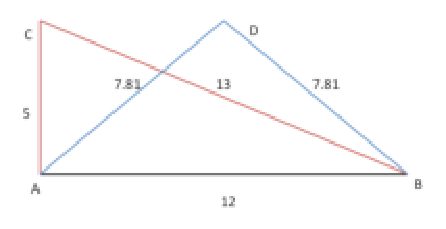
\includegraphics
    {Figures/CurvatureRatioTriangles.eps}}
  \caption{\label{CurvatureRatioTriangles} Caption}
\end{figure}

\noindent Additionally consider the triangle (\textit{A}, \textit{B}, 
\textit{D}) formed with the same base (12) and height (5) as the other 
triangle.  The perimeter of this triangle, (\textit{A}, \textit{B}, 
\textit{D}) is 27.62. Using point \textit{C} to increases the length of 
the segment locally by 150\%, while using point \textit{D} increases the 
length of the segment by 130.1\%.  Both of these triangles have the same 
curvature ratio since their bases and heights are identical.  However, as 
shown the perimeter can vary a not-insignificant amount without changing 
the curvature ratio of a segment.  Therefore, the curvature ratio is not 
sufficient to determine whether or not the arc-length of the discretization is approaching that of the curve—only that the distance between the discretization and the curve is approaching some value locally.  Using only the curvature ratio, the choice between point \textit{C} and \textit{D} in Figure-\ref{CurvatureRatioTriangles} are equal.  The potential error would get worse if the point \textit{C} were moved further left--demonstrating that the curvature ratio is not always a good indicator of discretization accuracy for curves that aren’t ``well-behaved'' between discrete segments.

